% Options for packages loaded elsewhere
\PassOptionsToPackage{unicode}{hyperref}
\PassOptionsToPackage{hyphens}{url}
\PassOptionsToPackage{dvipsnames,svgnames,x11names}{xcolor}
%
\documentclass[
  letterpaper,
  DIV=11,
  numbers=noendperiod]{scrartcl}

\usepackage{amsmath,amssymb}
\usepackage{iftex}
\ifPDFTeX
  \usepackage[T1]{fontenc}
  \usepackage[utf8]{inputenc}
  \usepackage{textcomp} % provide euro and other symbols
\else % if luatex or xetex
  \usepackage{unicode-math}
  \defaultfontfeatures{Scale=MatchLowercase}
  \defaultfontfeatures[\rmfamily]{Ligatures=TeX,Scale=1}
\fi
\usepackage{lmodern}
\ifPDFTeX\else  
    % xetex/luatex font selection
\fi
% Use upquote if available, for straight quotes in verbatim environments
\IfFileExists{upquote.sty}{\usepackage{upquote}}{}
\IfFileExists{microtype.sty}{% use microtype if available
  \usepackage[]{microtype}
  \UseMicrotypeSet[protrusion]{basicmath} % disable protrusion for tt fonts
}{}
\makeatletter
\@ifundefined{KOMAClassName}{% if non-KOMA class
  \IfFileExists{parskip.sty}{%
    \usepackage{parskip}
  }{% else
    \setlength{\parindent}{0pt}
    \setlength{\parskip}{6pt plus 2pt minus 1pt}}
}{% if KOMA class
  \KOMAoptions{parskip=half}}
\makeatother
\usepackage{xcolor}
\usepackage[top=30mm,left=20mm]{geometry}
\setlength{\emergencystretch}{3em} % prevent overfull lines
\setcounter{secnumdepth}{5}
% Make \paragraph and \subparagraph free-standing
\ifx\paragraph\undefined\else
  \let\oldparagraph\paragraph
  \renewcommand{\paragraph}[1]{\oldparagraph{#1}\mbox{}}
\fi
\ifx\subparagraph\undefined\else
  \let\oldsubparagraph\subparagraph
  \renewcommand{\subparagraph}[1]{\oldsubparagraph{#1}\mbox{}}
\fi

\usepackage{color}
\usepackage{fancyvrb}
\newcommand{\VerbBar}{|}
\newcommand{\VERB}{\Verb[commandchars=\\\{\}]}
\DefineVerbatimEnvironment{Highlighting}{Verbatim}{commandchars=\\\{\}}
% Add ',fontsize=\small' for more characters per line
\usepackage{framed}
\definecolor{shadecolor}{RGB}{243,245,246}
\newenvironment{Shaded}{\begin{snugshade}}{\end{snugshade}}
\newcommand{\AlertTok}[1]{\textcolor[rgb]{1.00,0.00,0.00}{\textbf{#1}}}
\newcommand{\AnnotationTok}[1]{\textcolor[rgb]{0.38,0.63,0.69}{\textbf{\textit{#1}}}}
\newcommand{\AttributeTok}[1]{\textcolor[rgb]{0.49,0.56,0.16}{#1}}
\newcommand{\BaseNTok}[1]{\textcolor[rgb]{0.25,0.63,0.44}{#1}}
\newcommand{\BuiltInTok}[1]{\textcolor[rgb]{0.00,0.50,0.00}{#1}}
\newcommand{\CharTok}[1]{\textcolor[rgb]{0.25,0.44,0.63}{#1}}
\newcommand{\CommentTok}[1]{\textcolor[rgb]{0.38,0.63,0.69}{\textit{#1}}}
\newcommand{\CommentVarTok}[1]{\textcolor[rgb]{0.38,0.63,0.69}{\textbf{\textit{#1}}}}
\newcommand{\ConstantTok}[1]{\textcolor[rgb]{0.53,0.00,0.00}{#1}}
\newcommand{\ControlFlowTok}[1]{\textcolor[rgb]{0.00,0.44,0.13}{\textbf{#1}}}
\newcommand{\DataTypeTok}[1]{\textcolor[rgb]{0.56,0.13,0.00}{#1}}
\newcommand{\DecValTok}[1]{\textcolor[rgb]{0.25,0.63,0.44}{#1}}
\newcommand{\DocumentationTok}[1]{\textcolor[rgb]{0.73,0.13,0.13}{\textit{#1}}}
\newcommand{\ErrorTok}[1]{\textcolor[rgb]{1.00,0.00,0.00}{\textbf{#1}}}
\newcommand{\ExtensionTok}[1]{\textcolor[rgb]{0.00,0.44,0.13}{#1}}
\newcommand{\FloatTok}[1]{\textcolor[rgb]{0.25,0.63,0.44}{#1}}
\newcommand{\FunctionTok}[1]{\textcolor[rgb]{0.02,0.16,0.49}{#1}}
\newcommand{\ImportTok}[1]{\textcolor[rgb]{0.00,0.50,0.00}{\textbf{#1}}}
\newcommand{\InformationTok}[1]{\textcolor[rgb]{0.38,0.63,0.69}{\textbf{\textit{#1}}}}
\newcommand{\KeywordTok}[1]{\textcolor[rgb]{0.00,0.44,0.13}{\textbf{#1}}}
\newcommand{\NormalTok}[1]{\textcolor[rgb]{0.00,0.44,0.13}{#1}}
\newcommand{\OperatorTok}[1]{\textcolor[rgb]{0.40,0.40,0.40}{#1}}
\newcommand{\OtherTok}[1]{\textcolor[rgb]{0.00,0.44,0.13}{#1}}
\newcommand{\PreprocessorTok}[1]{\textcolor[rgb]{0.74,0.48,0.00}{#1}}
\newcommand{\RegionMarkerTok}[1]{\textcolor[rgb]{0.00,0.44,0.13}{#1}}
\newcommand{\SpecialCharTok}[1]{\textcolor[rgb]{0.25,0.44,0.63}{#1}}
\newcommand{\SpecialStringTok}[1]{\textcolor[rgb]{0.73,0.40,0.53}{#1}}
\newcommand{\StringTok}[1]{\textcolor[rgb]{0.25,0.44,0.63}{#1}}
\newcommand{\VariableTok}[1]{\textcolor[rgb]{0.10,0.09,0.49}{#1}}
\newcommand{\VerbatimStringTok}[1]{\textcolor[rgb]{0.25,0.44,0.63}{#1}}
\newcommand{\WarningTok}[1]{\textcolor[rgb]{0.38,0.63,0.69}{\textbf{\textit{#1}}}}

\providecommand{\tightlist}{%
  \setlength{\itemsep}{0pt}\setlength{\parskip}{0pt}}\usepackage{longtable,booktabs,array}
\usepackage{calc} % for calculating minipage widths
% Correct order of tables after \paragraph or \subparagraph
\usepackage{etoolbox}
\makeatletter
\patchcmd\longtable{\par}{\if@noskipsec\mbox{}\fi\par}{}{}
\makeatother
% Allow footnotes in longtable head/foot
\IfFileExists{footnotehyper.sty}{\usepackage{footnotehyper}}{\usepackage{footnote}}
\makesavenoteenv{longtable}
\usepackage{graphicx}
\makeatletter
\def\maxwidth{\ifdim\Gin@nat@width>\linewidth\linewidth\else\Gin@nat@width\fi}
\def\maxheight{\ifdim\Gin@nat@height>\textheight\textheight\else\Gin@nat@height\fi}
\makeatother
% Scale images if necessary, so that they will not overflow the page
% margins by default, and it is still possible to overwrite the defaults
% using explicit options in \includegraphics[width, height, ...]{}
\setkeys{Gin}{width=\maxwidth,height=\maxheight,keepaspectratio}
% Set default figure placement to htbp
\makeatletter
\def\fps@figure{htbp}
\makeatother

\KOMAoption{captions}{tableheading}
\makeatletter
\makeatother
\makeatletter
\makeatother
\makeatletter
\@ifpackageloaded{caption}{}{\usepackage{caption}}
\AtBeginDocument{%
\ifdefined\contentsname
  \renewcommand*\contentsname{Table of contents}
\else
  \newcommand\contentsname{Table of contents}
\fi
\ifdefined\listfigurename
  \renewcommand*\listfigurename{List of Figures}
\else
  \newcommand\listfigurename{List of Figures}
\fi
\ifdefined\listtablename
  \renewcommand*\listtablename{List of Tables}
\else
  \newcommand\listtablename{List of Tables}
\fi
\ifdefined\figurename
  \renewcommand*\figurename{Figure}
\else
  \newcommand\figurename{Figure}
\fi
\ifdefined\tablename
  \renewcommand*\tablename{Table}
\else
  \newcommand\tablename{Table}
\fi
}
\@ifpackageloaded{float}{}{\usepackage{float}}
\floatstyle{ruled}
\@ifundefined{c@chapter}{\newfloat{codelisting}{h}{lop}}{\newfloat{codelisting}{h}{lop}[chapter]}
\floatname{codelisting}{Listing}
\newcommand*\listoflistings{\listof{codelisting}{List of Listings}}
\makeatother
\makeatletter
\@ifpackageloaded{caption}{}{\usepackage{caption}}
\@ifpackageloaded{subcaption}{}{\usepackage{subcaption}}
\makeatother
\makeatletter
\makeatother
\ifLuaTeX
  \usepackage{selnolig}  % disable illegal ligatures
\fi
\IfFileExists{bookmark.sty}{\usepackage{bookmark}}{\usepackage{hyperref}}
\IfFileExists{xurl.sty}{\usepackage{xurl}}{} % add URL line breaks if available
\urlstyle{same} % disable monospaced font for URLs
\hypersetup{
  pdftitle={Modeling 3},
  pdfauthor={Emi Cervantes},
  colorlinks=true,
  linkcolor={blue},
  filecolor={Maroon},
  citecolor={Blue},
  urlcolor={Blue},
  pdfcreator={LaTeX via pandoc}}

\title{Modeling 3}
\author{Emi Cervantes}
\date{2023-07-17}

\begin{document}
\maketitle
\renewcommand*\contentsname{Table of contents}
{
\hypersetup{linkcolor=}
\setcounter{tocdepth}{3}
\tableofcontents
}
\hypertarget{modeling-final-part-i}{%
\section{Modeling (Final PART I)}\label{modeling-final-part-i}}

\hypertarget{load-libraries}{%
\section{Load Libraries}\label{load-libraries}}

\begin{Shaded}
\begin{Highlighting}[]
\FunctionTok{library}\NormalTok{(tidyverse)}
\end{Highlighting}
\end{Shaded}

\begin{verbatim}
-- Attaching core tidyverse packages ------------------------ tidyverse 2.0.0 --
v dplyr     1.1.2     v readr     2.1.4
v forcats   1.0.0     v stringr   1.5.0
v ggplot2   3.4.2     v tibble    3.2.1
v lubridate 1.9.2     v tidyr     1.3.0
v purrr     1.0.1     
-- Conflicts ------------------------------------------ tidyverse_conflicts() --
x dplyr::filter() masks stats::filter()
x dplyr::lag()    masks stats::lag()
i Use the ]8;;http://conflicted.r-lib.org/conflicted package]8;; to force all conflicts to become errors
\end{verbatim}

\begin{Shaded}
\begin{Highlighting}[]
\FunctionTok{library}\NormalTok{(sjPlot)}
\end{Highlighting}
\end{Shaded}

\begin{verbatim}
Learn more about sjPlot with 'browseVignettes("sjPlot")'.
\end{verbatim}

\begin{Shaded}
\begin{Highlighting}[]
\FunctionTok{library}\NormalTok{(sjmisc)}
\end{Highlighting}
\end{Shaded}

\begin{verbatim}
Learn more about sjmisc with 'browseVignettes("sjmisc")'.

Attaching package: 'sjmisc'

The following object is masked from 'package:purrr':

    is_empty

The following object is masked from 'package:tidyr':

    replace_na

The following object is masked from 'package:tibble':

    add_case
\end{verbatim}

\begin{Shaded}
\begin{Highlighting}[]
\FunctionTok{library}\NormalTok{(sjlabelled)}
\end{Highlighting}
\end{Shaded}

\begin{verbatim}

Attaching package: 'sjlabelled'

The following object is masked from 'package:forcats':

    as_factor

The following object is masked from 'package:dplyr':

    as_label

The following object is masked from 'package:ggplot2':

    as_label
\end{verbatim}

\hypertarget{load-dataset}{%
\section{Load Dataset}\label{load-dataset}}

\begin{Shaded}
\begin{Highlighting}[]
\NormalTok{df }\OtherTok{\textless{}{-}}\NormalTok{ readxl}\SpecialCharTok{::}\FunctionTok{read\_xlsx}\NormalTok{(}\StringTok{\textquotesingle{}../../../data/math{-}anxiety{-}raw{-}data.xlsx\textquotesingle{}}\NormalTok{)}
\end{Highlighting}
\end{Shaded}

\begin{verbatim}
New names:
* `Subject ID #` -> `Subject ID #...8`
* `Subject ID #` -> `Subject ID #...9`
* `StartDate` -> `StartDate...11`
* `EndDate` -> `EndDate...12`
* `Progress` -> `Progress...13`
* `Duration (in seconds)` -> `Duration (in seconds)...17`
* `Finished` -> `Finished...18`
* `RecordedDate` -> `RecordedDate...19`
* `Browser_info_Browser` -> `Browser_info_Browser...20`
* `Browser_info_Version` -> `Browser_info_Version...21`
* `Browser_info_Operating System` -> `Browser_info_Operating System...22`
* `Browser_info_Resolution` -> `Browser_info_Resolution...23`
* `Misc_0` -> `Misc_0...36`
* `Misc_1` -> `Misc_1...100`
* `Misc_2` -> `Misc_2...145`
* `MW_control_1` -> `MW_control_1...210`
* `MW_control_2` -> `MW_control_2...211`
* `MW_control_3` -> `MW_control_3...212`
* `MW_control_4` -> `MW_control_4...213`
* `MW_control_5` -> `MW_control_5...214`
* `` -> `...219`
* `StartDate` -> `StartDate...221`
* `EndDate` -> `EndDate...222`
* `Progress` -> `Progress...223`
* `Duration (in seconds)` -> `Duration (in seconds)...224`
* `Finished` -> `Finished...225`
* `RecordedDate` -> `RecordedDate...226`
* `Browser_info_Browser` -> `Browser_info_Browser...227`
* `Browser_info_Version` -> `Browser_info_Version...228`
* `Browser_info_Operating System` -> `Browser_info_Operating System...229`
* `Browser_info_Resolution` -> `Browser_info_Resolution...230`
* `Misc_0` -> `Misc_0...232`
* `Misc_1` -> `Misc_1...239`
* `Misc_2` -> `Misc_2...290`
* `MW_control_1` -> `MW_control_1...295`
* `MW_control_2` -> `MW_control_2...296`
* `MW_control_3` -> `MW_control_3...297`
* `MW_control_4` -> `MW_control_4...298`
* `MW_control_5` -> `MW_control_5...299`
\end{verbatim}

\hypertarget{clean-dataset}{%
\subsection{Clean Dataset}\label{clean-dataset}}

\begin{Shaded}
\begin{Highlighting}[]
\NormalTok{tma\_lst }\OtherTok{\textless{}{-}} \FunctionTok{c}\NormalTok{(}\StringTok{"TMA\_1"}\NormalTok{, }\StringTok{"TMA\_2"}\NormalTok{, }\StringTok{"TMA\_3"}\NormalTok{,}\StringTok{"TMA\_4"}\NormalTok{, }\StringTok{"TMA\_5"}\NormalTok{, }\StringTok{"TMA\_6"}\NormalTok{,}
             \StringTok{"TMA\_sum"}\NormalTok{, }\StringTok{"TMA\_avg"}\NormalTok{)}
\NormalTok{df1 }\OtherTok{\textless{}{-}}\NormalTok{ df }\SpecialCharTok{\%\textgreater{}\%} \FunctionTok{select}\NormalTok{(Condition, Sex, chicago, nonwhite, pretest,}
\NormalTok{              MW\_day1\_avg, MW\_day2\_avg, SI\_avg, tma\_lst,}
\NormalTok{              Understand\_avg, Del\_OverallAcc)}
\end{Highlighting}
\end{Shaded}

\begin{verbatim}
Warning: Using an external vector in selections was deprecated in tidyselect 1.1.0.
i Please use `all_of()` or `any_of()` instead.
  # Was:
  data %>% select(tma_lst)

  # Now:
  data %>% select(all_of(tma_lst))

See <https://tidyselect.r-lib.org/reference/faq-external-vector.html>.
\end{verbatim}

\begin{Shaded}
\begin{Highlighting}[]
\CommentTok{\# Get rid of row that has NA values in Condition and/or Sex}
\NormalTok{df1 }\OtherTok{\textless{}{-}}\NormalTok{ df1 }\SpecialCharTok{\%\textgreater{}\%} \FunctionTok{filter}\NormalTok{(Condition }\SpecialCharTok{==} \DecValTok{1} \SpecialCharTok{|}\NormalTok{ Condition }\SpecialCharTok{==} \DecValTok{2}\NormalTok{)}
\NormalTok{df1 }\OtherTok{\textless{}{-}}\NormalTok{ df1 }\SpecialCharTok{\%\textgreater{}\%} \FunctionTok{filter}\NormalTok{(}\SpecialCharTok{!}\FunctionTok{is.na}\NormalTok{(Sex))}
\NormalTok{df1}\SpecialCharTok{$}\NormalTok{Condition[df1}\SpecialCharTok{$}\NormalTok{Condition }\SpecialCharTok{==} \DecValTok{2}\NormalTok{] }\OtherTok{\textless{}{-}} \DecValTok{0}
\CommentTok{\# Assign 0 for "boy" and 1 for "girl"}
\NormalTok{df1}\SpecialCharTok{$}\NormalTok{Sex[df1}\SpecialCharTok{$}\NormalTok{Sex }\SpecialCharTok{==} \DecValTok{1}\NormalTok{] }\OtherTok{\textless{}{-}} \DecValTok{0}
\NormalTok{df1}\SpecialCharTok{$}\NormalTok{Sex[df1}\SpecialCharTok{$}\NormalTok{Sex }\SpecialCharTok{==} \DecValTok{2}\NormalTok{] }\OtherTok{\textless{}{-}} \DecValTok{1}
\CommentTok{\# Make sure variable is categorical}
\NormalTok{df1}\SpecialCharTok{$}\NormalTok{chicago }\OtherTok{\textless{}{-}} \FunctionTok{as.factor}\NormalTok{(df1}\SpecialCharTok{$}\NormalTok{chicago)}
\NormalTok{df1}\SpecialCharTok{$}\NormalTok{Sex }\OtherTok{\textless{}{-}} \FunctionTok{as.factor}\NormalTok{(df1}\SpecialCharTok{$}\NormalTok{Sex)}
\end{Highlighting}
\end{Shaded}

\hypertarget{math-anxiety-by-gender-and-group}{%
\section{Math Anxiety by Gender and
Group}\label{math-anxiety-by-gender-and-group}}

\begin{Shaded}
\begin{Highlighting}[]
\NormalTok{cond }\OtherTok{\textless{}{-}} \FunctionTok{c}\NormalTok{(}\StringTok{"No Worked EX"}\NormalTok{, }\StringTok{"Worked EX"}\NormalTok{)}
\FunctionTok{names}\NormalTok{(cond) }\OtherTok{\textless{}{-}} \FunctionTok{c}\NormalTok{(}\DecValTok{0}\NormalTok{, }\DecValTok{1}\NormalTok{)}
\NormalTok{location }\OtherTok{\textless{}{-}} \FunctionTok{c}\NormalTok{(}\StringTok{"Irvine"}\NormalTok{, }\StringTok{"Chicago"}\NormalTok{)}
\FunctionTok{names}\NormalTok{(location) }\OtherTok{\textless{}{-}} \FunctionTok{c}\NormalTok{(}\DecValTok{0}\NormalTok{, }\DecValTok{1}\NormalTok{)}

\NormalTok{df1 }\SpecialCharTok{\%\textgreater{}\%} \FunctionTok{ggplot}\NormalTok{(}\FunctionTok{aes}\NormalTok{(}\AttributeTok{x =}\NormalTok{ TMA\_avg, }\AttributeTok{fill =}\NormalTok{ Sex,}
                   \AttributeTok{color =}\NormalTok{ Sex)) }\SpecialCharTok{+}
  \FunctionTok{geom\_density}\NormalTok{(}\AttributeTok{alpha =} \FloatTok{0.5}\NormalTok{) }\SpecialCharTok{+}
  \FunctionTok{theme\_minimal}\NormalTok{() }\SpecialCharTok{+}
  \FunctionTok{facet\_grid}\NormalTok{(}\AttributeTok{cols =} \FunctionTok{vars}\NormalTok{(chicago),}
             \AttributeTok{labeller =} \FunctionTok{labeller}\NormalTok{(}\AttributeTok{chicago =}\NormalTok{ location)) }\SpecialCharTok{+}
  \FunctionTok{scale\_fill\_manual}\NormalTok{(}\AttributeTok{values =} \FunctionTok{c}\NormalTok{(}\StringTok{"\#F0E442"}\NormalTok{, }\StringTok{"\#56B4E9"}\NormalTok{), }\AttributeTok{labels =} \FunctionTok{c}\NormalTok{(}\StringTok{"Boy"}\NormalTok{, }\StringTok{"Girl"}\NormalTok{)) }\SpecialCharTok{+}
  \FunctionTok{scale\_color\_manual}\NormalTok{(}\AttributeTok{values =} \FunctionTok{c}\NormalTok{(}\StringTok{"\#F0E442"}\NormalTok{, }\StringTok{"\#56B4E9"}\NormalTok{), }\AttributeTok{labels =} \FunctionTok{c}\NormalTok{(}\StringTok{"Boy"}\NormalTok{, }\StringTok{"Girl"}\NormalTok{)) }\SpecialCharTok{+}
  \FunctionTok{labs}\NormalTok{(}\AttributeTok{x =} \StringTok{"Math Anxiety"}\NormalTok{, }\AttributeTok{y =} \StringTok{"Density"}\NormalTok{,}
       \AttributeTok{fill =} \StringTok{"Gender"}\NormalTok{, }\AttributeTok{color =} \StringTok{"Gender"}\NormalTok{)}
\end{Highlighting}
\end{Shaded}

\begin{figure}[H]

{\centering 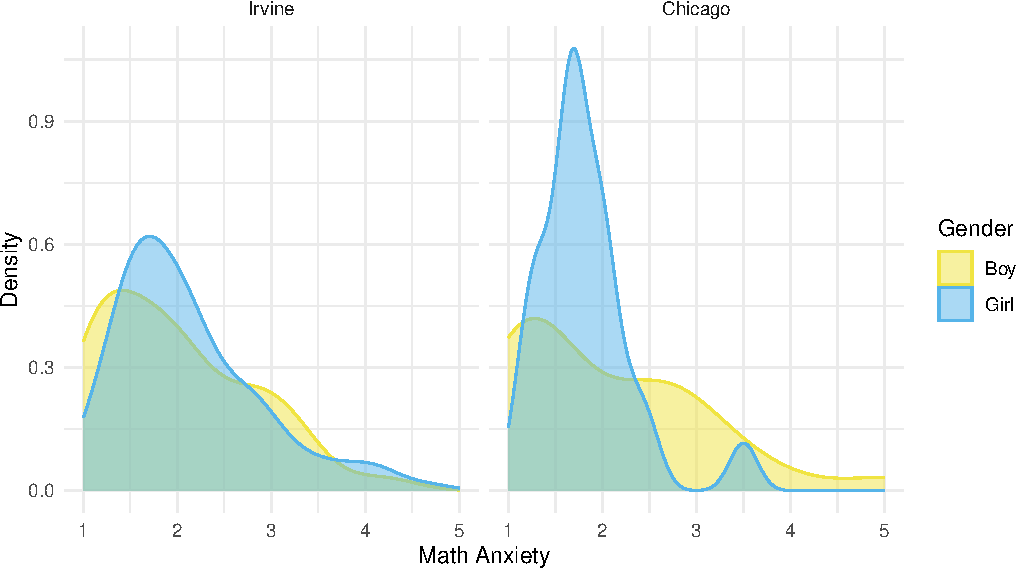
\includegraphics{modeling3_files/figure-pdf/unnamed-chunk-4-1.pdf}

}

\end{figure}

\begin{Shaded}
\begin{Highlighting}[]
\NormalTok{mu }\OtherTok{\textless{}{-}}\NormalTok{ df1 }\SpecialCharTok{\%\textgreater{}\%} \FunctionTok{group\_by}\NormalTok{(chicago, Condition, Sex) }\SpecialCharTok{\%\textgreater{}\%} \FunctionTok{summarize}\NormalTok{(}\AttributeTok{mean =} \FunctionTok{mean}\NormalTok{(TMA\_avg))}
\end{Highlighting}
\end{Shaded}

\begin{verbatim}
`summarise()` has grouped output by 'chicago', 'Condition'. You can override
using the `.groups` argument.
\end{verbatim}

\begin{Shaded}
\begin{Highlighting}[]
\NormalTok{tma\_hist\_plt }\OtherTok{\textless{}{-}}\NormalTok{ df1 }\SpecialCharTok{\%\textgreater{}\%} \FunctionTok{ggplot}\NormalTok{(}\FunctionTok{aes}\NormalTok{(}\AttributeTok{x =}\NormalTok{ TMA\_avg, }\AttributeTok{fill =}\NormalTok{ Sex,}
                   \AttributeTok{color =}\NormalTok{ Sex)) }\SpecialCharTok{+}
  \FunctionTok{geom\_density}\NormalTok{(}\AttributeTok{alpha =} \FloatTok{0.2}\NormalTok{) }\SpecialCharTok{+}
  \FunctionTok{theme\_minimal}\NormalTok{() }\SpecialCharTok{+}
  \FunctionTok{geom\_vline}\NormalTok{(}\AttributeTok{data=}\NormalTok{mu, }\FunctionTok{aes}\NormalTok{(}\AttributeTok{xintercept=}\NormalTok{mean, }\AttributeTok{color=}\NormalTok{Sex),}
           \AttributeTok{linetype=}\StringTok{"dashed"}\NormalTok{) }\SpecialCharTok{+}
  \FunctionTok{facet\_grid}\NormalTok{(}\AttributeTok{rows =} \FunctionTok{vars}\NormalTok{(Condition),}
             \AttributeTok{cols =} \FunctionTok{vars}\NormalTok{(chicago),}
             \AttributeTok{labeller =} \FunctionTok{labeller}\NormalTok{(}\AttributeTok{Condition =}\NormalTok{ cond,}
                                 \AttributeTok{chicago =}\NormalTok{ location)) }\SpecialCharTok{+}
  \FunctionTok{scale\_fill\_manual}\NormalTok{(}\AttributeTok{values =} \FunctionTok{c}\NormalTok{(}\StringTok{"\#FFC20A"}\NormalTok{, }\StringTok{"\#0C7BDC"}\NormalTok{), }\AttributeTok{labels =} \FunctionTok{c}\NormalTok{(}\StringTok{"Boy"}\NormalTok{, }\StringTok{"Girl"}\NormalTok{)) }\SpecialCharTok{+}
  \FunctionTok{scale\_color\_manual}\NormalTok{(}\AttributeTok{values =} \FunctionTok{c}\NormalTok{(}\StringTok{"\#FFC20A"}\NormalTok{, }\StringTok{"\#0C7BDC"}\NormalTok{), }\AttributeTok{labels =} \FunctionTok{c}\NormalTok{(}\StringTok{"Boy"}\NormalTok{, }\StringTok{"Girl"}\NormalTok{)) }\SpecialCharTok{+}
  \FunctionTok{labs}\NormalTok{(}\AttributeTok{x =} \StringTok{"Math Anxiety"}\NormalTok{, }\AttributeTok{y =} \StringTok{"Density"}\NormalTok{,}
       \AttributeTok{fill =} \StringTok{"Gender"}\NormalTok{, }\AttributeTok{color =} \StringTok{"Gender"}\NormalTok{) }\SpecialCharTok{+}\FunctionTok{theme}\NormalTok{(}\AttributeTok{legend.position=}\StringTok{"bottom"}\NormalTok{)}
\FunctionTok{ggsave}\NormalTok{(tma\_hist\_plt, }\AttributeTok{file =}  \StringTok{"../../../outputs/tma\_hist\_plt.png"}\NormalTok{,}
       \AttributeTok{width =} \DecValTok{8}\NormalTok{, }\AttributeTok{height =} \DecValTok{5}\NormalTok{)}
\NormalTok{tma\_hist\_plt}
\end{Highlighting}
\end{Shaded}

\begin{figure}[H]

{\centering 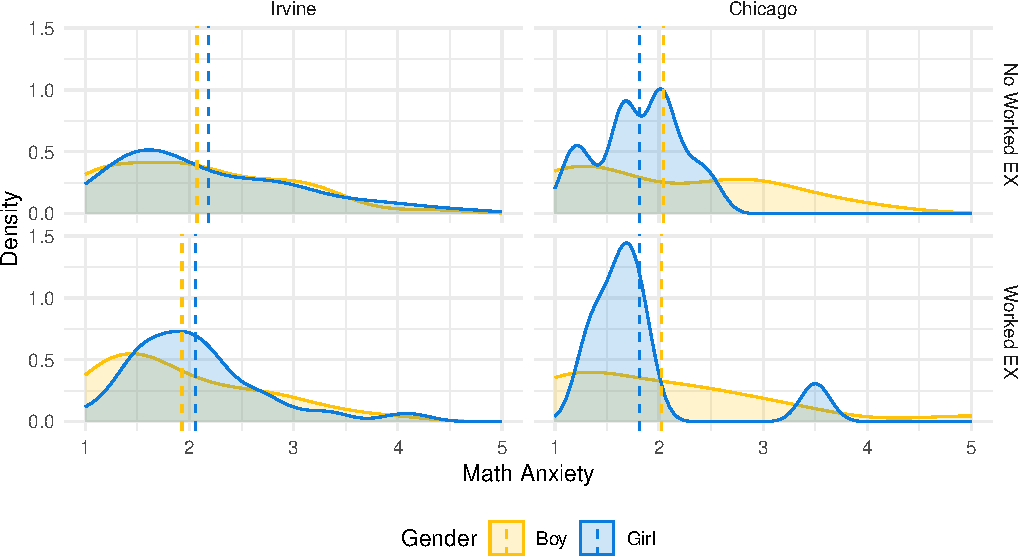
\includegraphics{modeling3_files/figure-pdf/unnamed-chunk-5-1.pdf}

}

\end{figure}

We see from the figure that in Irvine schools, girls seemed to have a
higher average math anxiety than boys in both condition. However, in
Chicago schools, boys seemed to have a higher math anxiety than girls in
both condition.

Girls seemed to have a higher math anxiety compared to boys overall.
Check if the difference is significant by using ANOVA test:

\begin{Shaded}
\begin{Highlighting}[]
\NormalTok{m1 }\OtherTok{\textless{}{-}} \FunctionTok{aov}\NormalTok{(TMA\_avg }\SpecialCharTok{\textasciitilde{}}\NormalTok{ Condition }\SpecialCharTok{+}\NormalTok{ chicago }\SpecialCharTok{+}\NormalTok{ Sex }\SpecialCharTok{+}\NormalTok{ Condition}\SpecialCharTok{*}\NormalTok{Sex, }
          \AttributeTok{data =}\NormalTok{ df1)}
\FunctionTok{summary}\NormalTok{(m1)}
\end{Highlighting}
\end{Shaded}

\begin{verbatim}
               Df Sum Sq Mean Sq F value Pr(>F)
Condition       1   0.52  0.5223   0.817  0.367
chicago         1   0.75  0.7512   1.175  0.279
Sex             1   0.08  0.0790   0.124  0.726
Condition:Sex   1   0.00  0.0007   0.001  0.974
Residuals     224 143.15  0.6391               
\end{verbatim}

No significant difference between gender on learning achievement and
math anxiety was found by gender.

\hypertarget{relationship-between-math-anxiety-and-learning-achievements}{%
\section{Relationship between Math Anxiety and Learning
Achievements}\label{relationship-between-math-anxiety-and-learning-achievements}}

\hypertarget{linear-regression}{%
\subsection{Linear Regression}\label{linear-regression}}

We will be fitting two different models to our data: one for predicting
\texttt{Del\_OverallAcc} and \texttt{Understand\_avg}.

\hypertarget{posttest-accuracy-scores}{%
\subsubsection{Posttest Accuracy
Scores}\label{posttest-accuracy-scores}}

\begin{Shaded}
\begin{Highlighting}[]
\CommentTok{\# Check if there\textquotesingle{}s any participant missing accuracy score data}
\NormalTok{df1 }\SpecialCharTok{\%\textgreater{}\%} \FunctionTok{count}\NormalTok{(}\FunctionTok{is.na}\NormalTok{(Del\_OverallAcc))}
\end{Highlighting}
\end{Shaded}

\begin{verbatim}
# A tibble: 1 x 2
  `is.na(Del_OverallAcc)`     n
  <lgl>                   <int>
1 FALSE                     229
\end{verbatim}

Every participant has a \texttt{Del\_OverallAcc} data, now we fit the
model to our data to predict \texttt{Del\_OverallAcc}:

\begin{Shaded}
\begin{Highlighting}[]
\CommentTok{\# Fit model}
\NormalTok{m2 }\OtherTok{\textless{}{-}}\NormalTok{ Del\_OverallAcc }\SpecialCharTok{\textasciitilde{}}\NormalTok{ TMA\_avg }\SpecialCharTok{+}\NormalTok{ MW\_day2\_avg }\SpecialCharTok{+}\NormalTok{ SI\_avg }\SpecialCharTok{+}\NormalTok{ chicago }\SpecialCharTok{+}\NormalTok{ Condition }\SpecialCharTok{+}\NormalTok{ Condition}\SpecialCharTok{*}\NormalTok{Sex }\SpecialCharTok{+}\NormalTok{ Condition}\SpecialCharTok{*}\NormalTok{TMA\_avg }\SpecialCharTok{+}\NormalTok{ Condition}\SpecialCharTok{*}\NormalTok{TMA\_avg}\SpecialCharTok{*}\NormalTok{Sex}
\NormalTok{fit2 }\OtherTok{\textless{}{-}} \FunctionTok{lm}\NormalTok{(m2, }\AttributeTok{data =}\NormalTok{ df1)}
\FunctionTok{summary}\NormalTok{(fit2)}
\end{Highlighting}
\end{Shaded}

\begin{verbatim}

Call:
lm(formula = m2, data = df1)

Residuals:
     Min       1Q   Median       3Q      Max 
-0.46538 -0.14589  0.01385  0.13172  0.45656 

Coefficients:
                         Estimate Std. Error t value Pr(>|t|)    
(Intercept)              0.788237   0.103465   7.618 7.76e-13 ***
TMA_avg                 -0.074960   0.035766  -2.096   0.0372 *  
MW_day2_avg             -0.013978   0.015217  -0.919   0.3593    
SI_avg                   0.023579   0.015840   1.489   0.1380    
chicago1                -0.247140   0.033346  -7.411 2.72e-12 ***
Condition1              -0.227621   0.102029  -2.231   0.0267 *  
Sex1                    -0.004203   0.104076  -0.040   0.9678    
Condition1:Sex1          0.115987   0.148327   0.782   0.4351    
TMA_avg:Condition1       0.117154   0.046947   2.495   0.0133 *  
TMA_avg:Sex1            -0.011958   0.046340  -0.258   0.7966    
TMA_avg:Condition1:Sex1 -0.066023   0.067743  -0.975   0.3308    
---
Signif. codes:  0 '***' 0.001 '**' 0.01 '*' 0.05 '.' 0.1 ' ' 1

Residual standard error: 0.1995 on 218 degrees of freedom
Multiple R-squared:  0.2576,    Adjusted R-squared:  0.2235 
F-statistic: 7.563 on 10 and 218 DF,  p-value: 2.516e-10
\end{verbatim}

\textbf{Significant Predictors}

\begin{itemize}
\item
  \texttt{TMA\_avg} (p = 0.0372): While controlling for other
  predictors, every 1 unit of increase in math anxiety decreases
  accuracy scores by 0.075.
\item
  \texttt{TMA\_avg:Condition} (p = 0.0133): Students who received worked
  examples, while controlling for other predictors, had increase in
  accuracy by 0.04 for every 1 unit increase in math anxiety.
\item
  Other significant predictors include: \texttt{chicago} (p = 2.72e-12),
  \texttt{Condition} (p = 0.0267)
\end{itemize}

\hypertarget{perceived-understanding}{%
\subsubsection{Perceived Understanding}\label{perceived-understanding}}

\begin{Shaded}
\begin{Highlighting}[]
\CommentTok{\# Check if there\textquotesingle{}s any participant missing understanding data}
\NormalTok{df1 }\SpecialCharTok{\%\textgreater{}\%} \FunctionTok{count}\NormalTok{(}\FunctionTok{is.na}\NormalTok{(Understand\_avg))}
\end{Highlighting}
\end{Shaded}

\begin{verbatim}
# A tibble: 2 x 2
  `is.na(Understand_avg)`     n
  <lgl>                   <int>
1 FALSE                     227
2 TRUE                        2
\end{verbatim}

2 participants were missing \texttt{Understand\_avg} data (row \#56 and
\#198)

\begin{Shaded}
\begin{Highlighting}[]
\CommentTok{\# Fill out missing understanding avg data with the group average}
\NormalTok{understand\_avg1 }\OtherTok{\textless{}{-}}\NormalTok{ df1 }\SpecialCharTok{\%\textgreater{}\%} \FunctionTok{filter}\NormalTok{(Condition }\SpecialCharTok{==} \DecValTok{1} \SpecialCharTok{\&}\NormalTok{ Sex }\SpecialCharTok{==} \DecValTok{0} \SpecialCharTok{\&}\NormalTok{ chicago }\SpecialCharTok{==} \DecValTok{0}\NormalTok{) }\SpecialCharTok{\%\textgreater{}\%} \FunctionTok{summarize}\NormalTok{(}\AttributeTok{mean\_understand =} \FunctionTok{mean}\NormalTok{(Understand\_avg, }\AttributeTok{na.rm =} \ConstantTok{TRUE}\NormalTok{))}
\NormalTok{understand\_avg2 }\OtherTok{\textless{}{-}}\NormalTok{ df1 }\SpecialCharTok{\%\textgreater{}\%} \FunctionTok{filter}\NormalTok{(Condition }\SpecialCharTok{==} \DecValTok{0} \SpecialCharTok{\&}\NormalTok{ Sex }\SpecialCharTok{==} \DecValTok{0} \SpecialCharTok{\&}\NormalTok{ chicago }\SpecialCharTok{==} \DecValTok{0}\NormalTok{) }\SpecialCharTok{\%\textgreater{}\%} \FunctionTok{summarize}\NormalTok{(}\AttributeTok{mean\_understand =} \FunctionTok{mean}\NormalTok{(Understand\_avg, }\AttributeTok{na.rm =} \ConstantTok{TRUE}\NormalTok{))}
\CommentTok{\# assign imputed value}
\NormalTok{df1[}\DecValTok{56}\NormalTok{, }\DecValTok{17}\NormalTok{] }\OtherTok{=}\NormalTok{ understand\_avg1}
\NormalTok{df1[}\DecValTok{198}\NormalTok{, }\DecValTok{17}\NormalTok{] }\OtherTok{=}\NormalTok{ understand\_avg1}
\end{Highlighting}
\end{Shaded}

Every participant now has a \texttt{Understand\_avg} data, now we fit
the model to our data to predict \texttt{Understand\_avg}:

\begin{Shaded}
\begin{Highlighting}[]
\NormalTok{m3 }\OtherTok{\textless{}{-}}\NormalTok{ Understand\_avg }\SpecialCharTok{\textasciitilde{}}\NormalTok{ TMA\_avg }\SpecialCharTok{+}\NormalTok{ MW\_day2\_avg }\SpecialCharTok{+}\NormalTok{ SI\_avg }\SpecialCharTok{+}\NormalTok{ chicago }\SpecialCharTok{+}\NormalTok{ Condition }\SpecialCharTok{+}\NormalTok{ Condition}\SpecialCharTok{*}\NormalTok{Sex }\SpecialCharTok{+}\NormalTok{ Condition}\SpecialCharTok{*}\NormalTok{TMA\_avg }\SpecialCharTok{+}\NormalTok{ Condition}\SpecialCharTok{*}\NormalTok{TMA\_avg}\SpecialCharTok{*}\NormalTok{Sex}
\NormalTok{fit3 }\OtherTok{\textless{}{-}} \FunctionTok{lm}\NormalTok{(m3, }\AttributeTok{data =}\NormalTok{ df1)}
\FunctionTok{summary}\NormalTok{(fit3)}
\end{Highlighting}
\end{Shaded}

\begin{verbatim}

Call:
lm(formula = m3, data = df1)

Residuals:
    Min      1Q  Median      3Q     Max 
-61.937 -10.233   4.723  12.935  44.362 

Coefficients:
                        Estimate Std. Error t value Pr(>|t|)    
(Intercept)              70.6464    10.2858   6.868 6.69e-11 ***
TMA_avg                  -0.6890     3.5556  -0.194 0.846526    
MW_day2_avg              -6.2254     1.5128  -4.115 5.49e-05 ***
SI_avg                    7.0573     1.5747   4.482 1.20e-05 ***
chicago1                -11.5941     3.3150  -3.497 0.000569 ***
Condition1               -1.6788    10.1430  -0.166 0.868697    
Sex1                      1.8821    10.3465   0.182 0.855824    
Condition1:Sex1           4.8053    14.7456   0.326 0.744826    
TMA_avg:Condition1       -1.0156     4.6671  -0.218 0.827933    
TMA_avg:Sex1             -2.3541     4.6068  -0.511 0.609857    
TMA_avg:Condition1:Sex1   0.6709     6.7345   0.100 0.920735    
---
Signif. codes:  0 '***' 0.001 '**' 0.01 '*' 0.05 '.' 0.1 ' ' 1

Residual standard error: 19.84 on 218 degrees of freedom
Multiple R-squared:  0.2522,    Adjusted R-squared:  0.2178 
F-statistic:  7.35 on 10 and 218 DF,  p-value: 5.119e-10
\end{verbatim}

\textbf{Significant Predictors}

\begin{itemize}
\item
  \texttt{MW\_day2\_avg} (p = 5.49e-05): While controlling for other
  predictors, every 1 unit of increase in mind wandering decreases
  perceived understanding by 6.2254.
\item
  \texttt{SI\_avg} (p = 1.20e-05): While controlling for other
  predictors, every 1 unit of increase in situational interest decreases
  perceived understanding by 7.0573.
\item
  \texttt{chicago} (p = 0.00056)
\end{itemize}

\begin{Shaded}
\begin{Highlighting}[]
\CommentTok{\# Display result as a table}
\FunctionTok{tab\_model}\NormalTok{(fit2, fit3,}
          \AttributeTok{pred.labels =} \FunctionTok{c}\NormalTok{(}\StringTok{"Intercept"}\NormalTok{, }\StringTok{"Math }
\StringTok{                          Anxiety"}\NormalTok{, }\StringTok{"Mind }
\StringTok{                          Wandering"}\NormalTok{, }
                          \StringTok{"Situational }
\StringTok{                          Interest"}\NormalTok{, }\StringTok{"Site (Chicago)"}\NormalTok{, }\StringTok{"Condition (Worked EX)"}\NormalTok{, }\StringTok{"Gender (boy)"}\NormalTok{, }\StringTok{"Condition (Worked EX)*Gender (boy)"}\NormalTok{, }\StringTok{"Math Anxiety*Condition (Worked EX)"}\NormalTok{, }\StringTok{"Math Anxiety*Gender (boy)"}\NormalTok{, }\StringTok{"Math Anxiety*Condition (Worked EX)*Gender (boy)"}\NormalTok{),}
  \AttributeTok{dv.labels =} \FunctionTok{c}\NormalTok{(}\StringTok{"Posttest Accuracy"}\NormalTok{, }\StringTok{"Perceived Understanding"}\NormalTok{))}
\end{Highlighting}
\end{Shaded}

\begin{longtable}[]{@{}ccccccc@{}}
\toprule\noalign{}
\endhead
\bottomrule\noalign{}
\endlastfoot
~ &
\multicolumn{3}{>{\centering\arraybackslash}p{(\columnwidth - 12\tabcolsep) * \real{0.0000} + 4\tabcolsep}}{%
Posttest Accuracy} &
\multicolumn{3}{>{\centering\arraybackslash}p{(\columnwidth - 12\tabcolsep) * \real{0.0000} + 4\tabcolsep}@{}}{%
Perceived Understanding} \\
Predictors & Estimates & CI & p & Estimates & CI & p \\
Intercept & 0.79 & 0.58~--~0.99 & \textbf{\textless0.001} & 70.65 &
50.37~--~90.92 & \textbf{\textless0.001} \\
Math Anxiety & -0.07 & -0.15~--~-0.00 & \textbf{0.037} & -0.69 &
-7.70~--~6.32 & 0.847 \\
Mind Wandering & -0.01 & -0.04~--~0.02 & 0.359 & -6.23 & -9.21~--~-3.24
& \textbf{\textless0.001} \\
Situational Interest & 0.02 & -0.01~--~0.05 & 0.138 & 7.06 &
3.95~--~10.16 & \textbf{\textless0.001} \\
Site (Chicago) & -0.25 & -0.31~--~-0.18 & \textbf{\textless0.001} &
-11.59 & -18.13~--~-5.06 & \textbf{0.001} \\
Condition (Worked EX) & -0.23 & -0.43~--~-0.03 & \textbf{0.027} & -1.68
& -21.67~--~18.31 & 0.869 \\
Gender (boy) & -0.00 & -0.21~--~0.20 & 0.968 & 1.88 & -18.51~--~22.27 &
0.856 \\
Condition (Worked EX)*Gender (boy) & 0.12 & -0.18~--~0.41 & 0.435 & 4.81
& -24.26~--~33.87 & 0.745 \\
Math Anxiety*Condition (Worked EX) & 0.12 & 0.02~--~0.21 &
\textbf{0.013} & -1.02 & -10.21~--~8.18 & 0.828 \\
Math Anxiety*Gender (boy) & -0.01 & -0.10~--~0.08 & 0.797 & -2.35 &
-11.43~--~6.73 & 0.610 \\
Math Anxiety*Condition (Worked EX)*Gender (boy) & -0.07 & -0.20~--~0.07
& 0.331 & 0.67 & -12.60~--~13.94 & 0.921 \\
Observations &
\multicolumn{3}{>{\raggedright\arraybackslash}p{(\columnwidth - 12\tabcolsep) * \real{0.0000} + 4\tabcolsep}}{%
229} &
\multicolumn{3}{>{\raggedright\arraybackslash}p{(\columnwidth - 12\tabcolsep) * \real{0.0000} + 4\tabcolsep}@{}}{%
229} \\
R\textsuperscript{2} / R\textsuperscript{2} adjusted &
\multicolumn{3}{>{\raggedright\arraybackslash}p{(\columnwidth - 12\tabcolsep) * \real{0.0000} + 4\tabcolsep}}{%
0.258 / 0.224} &
\multicolumn{3}{>{\raggedright\arraybackslash}p{(\columnwidth - 12\tabcolsep) * \real{0.0000} + 4\tabcolsep}@{}}{%
0.252 / 0.218} \\
\end{longtable}

\hypertarget{results}{%
\section{Results}\label{results}}

\begin{itemize}
\item
  No significant effect was found by gender on either math anxiety or
  learning achievements
\item
  However, we saw that worked examples were overall effective in
  reducing the effect of math anxiety on posttest accuracy scores,
  regardless of gender and sites
\item
  No significant effect was found by math anxiety on perceived
  understanding. Instead, mind wandering and situational interest were
  two dominant significant predictors.
\item
  Students in Chicago significantly performed worst in learning
  achievements
\end{itemize}



\end{document}
